\chapter{Mitigate Fingerprint Activities of Honeypots}
\label{chap:fingerprinting}

\epigraph{There is a generic weakness in the current generation of low- and medium-interaction honeypots because of their reliance on off-the-shelf libraries to implement large parts of the transport layer.}{\textit{Alexander Vetterl}}

Detecting honeypots before launching attacks helps to avoid the disclosure of information.
The \autoref{chap:cloud-security} has shown that bot activities are on the rise, and more attacks than ever have been launched.
However, the vast majority of attacks have been identified to be repetitive.
This chapter conducts two experiments on whether it is possible to fingerprint honeypots.
First, it reproduces the findings that \citet{vetterl2020} claims to prove the initial question if any fingerprint activity is feasible.
Lastly, it presents a concept to disguise Cowrie and verify this assumption with an experiment.

\section{OpenSSH}
\label{sec:openssh}

OpenSSH is one of the most used applications that enables SSH.
Before proceeding with generic weaknesses of honeypots, a short intermezzo about OpenSSH is given.

\begin{figure}
    \centering
    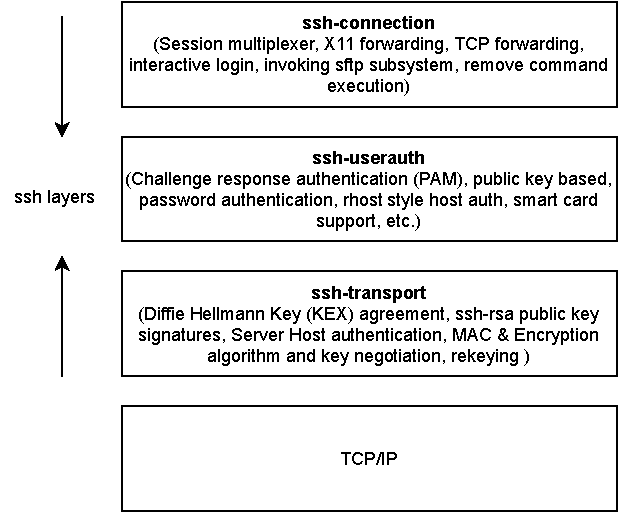
\includegraphics{figures/openssh-architecture.pdf}
    \caption[OpenSSH architecture]{
        OpenSSH architecture (derived from \cite{openssh2007}).
        The ssh-transport layer builds the foundation for the other layers on top.
        In addition, each layer lists examples of functionalities that it supports. 
    }
    \label{fig:openssh-architecture}
\end{figure}

OpenSSH consists of three major layers, namely \verb|ssh-connection|, \verb|ssh-userauth|, and \verb|ssh-transport| (\autoref{fig:openssh-architecture}).
The last layer is the most important because it provides the basic functionalities for crypto operations, such as key exchange and encryption.

The first layer is responsible for authenticating the user to the sshd daemon.
Based on two-way authentication, the client authenticates the sshd daemon with the help of the \verb|ssh-transport|.
Finally, a secure connection is established, and the key exchange is done.
The next step is to authenticate the user of the client.
It offers authentication methods such as username/password, public key, or smart-card authentication.
If the \verb|ssh-userauth| layer is successful, it will establish a secure channel through the \verb|ssh-connection| layer.
Each session is handled in a so-called channel.

The \verb|ssh-connection| layer handles multiple sessions simultaneously over a single \verb|ssh-userauth| layer with the TCP/IP layer below.
It is responsible for executing arbitrary commands, forwarding X11 connections, establishing VPN tunnels, and more.

In addition, OpenSSH has built-in features such as keeping alive messages and redirecting stdin to /dev/null for specialized X11 windows.

\autoref{fig:openssh-flow-diagram} outlines a sample session between a client and a server.
The key exchange initialization is the first message between them to negotiate all ciphers and keys for communication.
For this chapter, no other than this message will be considered.

\section{Preliminary Work}

Attackers have a solid motivation to reveal honeypots before launching an attack.
Without any protection, attackers would disclose their methods, and thus, newly developed attacks would become useless.
As shown in \autoref{chap:cloud-security}, attackers do try to get information about the host system.
\citet{vetterl2020} discussed various methods of fingerprinting; however, executing commands in a shell and examining the response leaves precarious information to the honeypot itself.
His technical report evaluated methods to detect honeypots at the transport level.
As stated, the value of a honeypot would be merely zero if detection on transport level would work.
He presents fingerprinting methods for SSH, Telnet, and HTTP/Web.
Due to the complexity of each method, this section focuses on SSH fingerprinting using the honeypot Cowrie.

The idea to detect SSH honeypots is to look for deviations in the response.
Therefore, \citet{vetterl2020} sends a set of probes $P = \{P_1, P_2, \dots, P_n\}$ to a given set of implementations of a network protocol $I = \{I_1, I_2, \dots, I_n\}$ and stores the set of responses $R = \{R_1, R_2, \dots, R_n\}$.
He calculated the cosine similarity coefficient $C$ for the given set of responses.
The goal is to find the best $P_i$ where the sum of $C$ is the lowest.
\autoref{fig:draft-cosine-similarity} presents these steps.

The cosine similarity outputs the similarity between vectors of numerical attributes.
It is widely used in text semantics to measure the similarity of sets of information such as two sentences.
\citet{vetterl2020} outlines that it can be used in \enquote{traffic analysis to find abnormalities and to measure domain similarity}.
Mathematically, it computes the angle between two vectors.
For each set of information $A$, we create a vector $D_A$.
Referring to the use case with SSH, we use the response from the server as information $A$.
If $\theta$ is the angle between $D_A$ and $D_B$, then:

\begin{equation} \label{eq:cosine-similarity}
    \cos \theta = \frac{D_A \cdot D_B}{\|D_A\| \|D_B\|}
\end{equation}

where \enquote{$\cdot$} is the dot product obtained by:

\begin{equation}
    D_A \cdot D_B = \sum_{i=1}^{n} (D_{A_i} \times D_{B_i})
\end{equation}

and $\|D_A\|$ (resp. $\|D_B\|$) is the Euclidean norm, obtained by $\sqrt{\sum_{i=1}^{n} D_{A_i}^2}$ (resp. $\sqrt{\sum_{i=1}^{n} D_{B_i}^2}$).
The values of vectors are non-negative.
The similarity between items is the value $\cos \theta$, $\cos \theta = 1$ indicates equality.

\begin{figure}
    \centering
    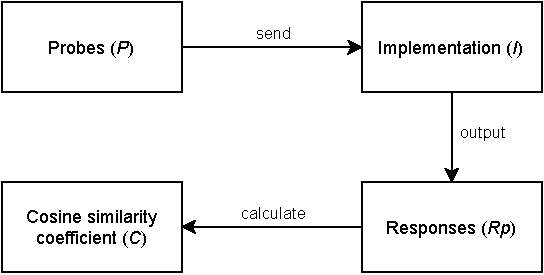
\includegraphics{figures/vetterl_concept.pdf}
    \caption[Outline to obtain the cosine similarity coefficient]{
        Outline to obtain the cosine similarity coefficient (derived from \cite{vetterl2020}).
    }
    \label{fig:draft-cosine-similarity}
\end{figure}

In order to find the best $P_i$ for SSH, \citet{vetterl2020} first created different SSH version strings based on the format: \verb|SSH-protoversion-swversion SP comment crlf|.
He used different lower and upper case variations, 12 different \textit{protoversions} ranging from $0.0$ to $3.2$, \textit{swversion} set to \enquote{OpenSSH} or empty string, \textit{comment} set to \enquote{FreeBSD} or empty string, and \textit{crlf} to either \verb|\r\n| or empty string.
In total, summing up to \numprint{192} client version strings.
Second, he created different \verb|SSH2_MSG_KEXINIT| packets with 16 key-exchange algorithms, two host key algorithms, 15 encryption algorithms, 5 MAC algorithms, and three compression algorithms.
In total, he sent \numprint{58,752} key exchange initialization messages.
Combining them with the \numprint{192} client versions, he ended up sending \numprint{157925376} packets.
The version string \verb|SSH-2.2-OpenSSH \r\n| and the \verb|SSH2_MSG_KEXINIT| packet including \textit{ecdh-sha2-nistp521} as the key-exchange algorithm, \textit{ssh-dss} as host key algorithm, \textit{blowfish-cbc} as encryption algorithm, \textit{hmac-sha1} as mac algorithm, and \textit{zlib@openssh.com} as compression algorithm, with the wrong padding, resulting in the lowest cosine similarity coefficient $C$.
\autoref{lst:ssh-debug} shows the SSH debug information with the modified version string and key exchange message.

\begin{figure}
    \lstinputlisting[language=bash, caption={[Example OpenSSH connection with probed SSH packet]OpenSSH connection attempt with probed SSH packet. All non-essential debug information have been removed to lay emphasis on the modified key exchange initialization.}, label={lst:ssh-debug}]{listings/ssh-debug.txt}
\end{figure}

\autoref{tab:cosine-similarity} has been derived from \citet{vetterl2020} to present his results of the cosine similarity of OpenSSH, Twisted, and Cowrie.
Twisted has been added to have an example with an older SSH honeypot.
As seen, it differs fundamentally from OpenSSH.
At most, it scores $0.52$ whereas various OpenSSH versions start at $0.98$.
The number of hosts significantly decreases with a cosine similarity score of $0.90$ and higher.
Cowrie responses are not too far away from OpenSSH, with an average of $0.80$.
However, scanning through the web with a minimum score of $0.90$ and higher would exclude all honeypots.
Thus, distinguishing Cowrie from OpenSSH with SSH packets is a feasible method.
Moreover, \citet{vetterl2020} performed an Internet-wide scan, and detected \numprint{758} Kippo and \numprint{2021} Cowrie honeypots.
These results show that the values of honeypots would decrease to zero when fingerprinting activities are used.

\begin{figure}
    \centering
    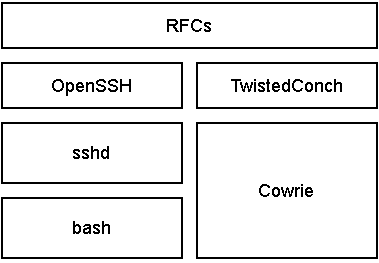
\includegraphics{figures/cowrie-openssh.pdf}
    \caption[Architecture of OpenSSH and Cowrie]{
        Architecture of OpenSSH and Cowrie.
        OpenSSH and TwistedConch have subtle protocol differences (derived from \cite{vetterl2020}).
    }
    \label{fig:cowrie-openssh}
\end{figure}

\citet{vetterl2020} states that current low- and medium-interaction honeypots have a generic weakness due to the underlying off-the-shelf libraries.
Cowrie is based on TwistedConch\footnote{\href{https://github.com/twisted/twisted/commit/4e3b22afe1f76b360733b65d6b835b7aaae6deb6}{TwistedConch 27.0.1} on GitHub}, a Python 2/3 library that implements the SSH protocol.
Any bash command and its response are tweaked by Cowrie, and thus, resulting in a discrepancy to OpenSSH.
For example, Cowrie version $1.1.0$ missed \verb|tftp|\footnote{Trivial File Transfer Protocol (TFTP) is a lockstep File Transfer Protocol} that later came with version $1.2.0$.
Therefore, it is a continuous struggle to add new commands to avoid early disclosures of Cowrie.

\autoref{fig:cowrie-openssh} shows the difference between OpenSSH and Cowrie.
Both have to fulfill the RFC4250 \cite{rfc4250} which defines the protocol.
OpenSSH and TwistedConch implement the RFC requirement.
As an example, \citet{vetterl2020} found that Cowrie used to have random bytes for the key exchange initialization packet\footnote{Each packet consists of the packet and padding length, the \ac{mac}, a payload, and random padding.}.
With respect to RFC4253 \cite{rfc4253} that defines the \ac{bpp} of SSH, the random padding is used to solidify the total length of the packet to be a multiple of the cipher block size.
The RFC in section 6 defines that the padding consists of 4 random bytes.
Based on the statement of the OpenSSH authors, random bytes have been changed to \verb|NULL| characters due to no security implications.
Thus, an adversary could have detected a Cowrie honeypot with a single key exchange initialization packet.
Nowadays, Cowrie adapted itself to have \verb|NULL| characters as padding to mitigate such an exploit.
However, these subtle differences give adversaries precautionary information and influence the cosine similarity coefficient.

\begin{table}
    \caption[Overview of the cosine similarity of OpenSSH, Cowrie, and Twisted]{
        Overview of the cosine similarity of OpenSSH, Cowrie, and Twisted.
        Twisted has been added to have a comparison to an older honeypot.
    }
    \begin{tabular}{lc|cccccccccc}
    \toprule
                   &   & A & B      & C      & D      & E      & F      & G      & H      & I      & J      \\
    \hline
    OpenSSH 6.6    & A & - & $0.98$ & $0.98$ & $0.94$ & $0.94$ & $0.42$ & $0.78$ & $0.79$ & $0.79$ & $0.79$ \\
    OpenSSH 6.7    & B &   & -      & $0.98$ & $0.98$ & $0.98$ & $0.41$ & $0.80$ & $0.81$ & $0.81$ & $0.80$ \\
    OpenSSH 6.8    & C &   &        & -      & $0.96$ & $0.96$ & $0.42$ & $0.78$ & $0.79$ & $0.79$ & $0.79$ \\
    OpenSSH 7.2    & D &   &        &        & -      & $0.98$ & $0.42$ & $0.80$ & $0.80$ & $0.80$ & $0.80$ \\
    OpenSSH 7.5    & E &   &        &        &        & -      & $0.42$ & $0.78$ & $0.79$ & $0.79$ & $0.79$ \\
    \\
    \cline{1-2} \cline{8-12}
    \\
    Twisted 15.2.1 & F &   &        &        &        &        & -      & $0.50$ & $0.51$ & $0.51$ & $0.52$ \\
    \\
    \cline{1-2} \cline{9-12}
    \\
    Cowrie 96ca2ba & G &   &        &        &        &        &        & -      & $0.98$ & $0.98$ & $0.98$ \\
    Cowrie dc45961 & H &   &        &        &        &        &        &        & -      & $0.99$ & $0.99$ \\
    Cowrie dbe88ed & I &   &        &        &        &        &        &        &        & -      & $0.99$ \\
    Cowrie fd801d1 & J &   &        &        &        &        &        &        &        &        & -      \\
    \bottomrule
    \end{tabular}
    \label{tab:cosine-similarity}
\end{table}

\section{Experiment 1: Reproduce Vetterl et al.'s findings}

First, the reproduction of the outdated OpenSSH library that \citet{vetterl2020} used will be investigated.
In his work, he used the version $7.5P1$, which deviates from the latest version $8.8P1$.
Older versions rely on OpenSSL $1.0.2$, including outdated algorithms and functions.
For the \verb|SSH2_MSG_KEXINIT| packet, the encryption algorithm \textit{blowfish-cbc} is outdated and has been removed with version $7.6P1$.
Building the version $7.5P1$ requires the libraries libssl ($1.0.2$), libssl-dev ($1.0$), libssh-dev ($0.7.3-2$), and libssh-4 ($0.9.6-1$).
All of these libraries are outdated and have been removed from any Debian installation.
Using the latest versions of these libraries results in missing encryption algorithms and host key algorithms.
Thus, replacing the libraries is a necessary task.
It is required to download the libraries, remove the current versions, and install the outdated ones.
The version $7.5P1$ allows modifying the key exchange initialization message proposal in a single file.
On the contrary, this has been removed starting from version $7.6P1$.
After compiling the application, its behavior has been tested with a Debian $11$ Buster and a Debian Jessie $9$ Docker image.
Both are new machines with no other installed packages than the sshd daemon.
Debian $11$ uses the latest OpenSSH version, whereas Jessie is at $6.7P1$.
These environments help to uniquely identify variations in the protocol version.

\begin{figure}
    \lstinputlisting[language=bash, caption={[OpenSSH connection attempt with probed message]OpenSSH connection attempt for version $7.5P1$ and $8.8P1$ with probed key exchange initialization message. All non-essential debug information have been removed to lay emphasis on the modified key exchange initialization.}, label={lst:ssh-openssh}]{listings/ssh-openssh.txt}
\end{figure}

\autoref{lst:ssh-openssh} shows the connection attempt with the adjusted version string and \verb|SSH2_MSG_KEXINIT| packet.
Both Debian machines return the same response.
Using the outdated version $7.5P1$ results in an incompatibility.
The return message outlines that \textit{blowfish-cbc} is not supported anymore.
OpenSSH kept the encryption algorithm usable for compatibility reasons for clients until $7.6P1$.
Later patches removed the \textit{blowfish-cbc} from the application; therefore, a reproduction of \citet{vetterl2020} remains not feasible with the latest version.
However, testing it with version $7.3P1$ that has been compiled on the machine results in a successful connection attempt.
\citet{vetterl2020} does not outline any expected response of OpenSSH; thus, it can be assumed that a connection attempt would have been successful due to the existing ciphers during that time.
Adapting the version $8.8P1$ with \textit{chacha20-poly1305} instead of \textit{blowfish-cbc} for the encryption algorithm results in a successful connection attempt.
Thus, the key exchange initialization has been adapted to use \textit{chacha20-poly1305} as encryption algorithm instead.
Next, the DSA host key algorithms are marked as too weak and are not included automatically during the key exchange initialization.
Using \textit{ssh-dss} requires the extra flag \verb|-oHostKeyAlgorithms=+ssh-dss|.
In order to avoid weak algorithms, the \textit{ssh-ed25519} host key algorithm is used, and the response has been promising to probe instances.
So far, the key exchange initialization packet with \textit{ecdh-sha2-nistp521} as key exchange algorithm, \textit{ssh-ed25519} as host key algorithm, \textit{chacha20-poly1305} as encryption algorithm, \textit{hmac-sha1} as mac algorithm, and \textit{zlib@openssh.com} as compression algorithm have been successfully tested on the two Debian instances.

\begin{figure}
    \lstinputlisting[language=bash, caption={[Cowrie connection attempt with probed message]Cowrie connection attempt with probed key exchange initialization message. All non-essential debug information have been removed to lay emphasis on the modified key exchange initialization.}, label={lst:ssh-cowrie}]{listings/ssh-cowrie.txt}
\end{figure}

The most interesting question remains about Cowrie's response deviation.
\citet{vetterl2020} claims that it results in a \verb|bad version *| exception.
Cowrie has fixed this issue in the meantime, and thus, it does not leak vulnerable information anymore.
For the experiment, the default Cowrie implementation version $v.2.3.0$\footnote{\href{https://github.com/cowrie/cowrie/commit/555ff10d95f6239d9d6efee8a2d05def316ab144}{Cowrie v2.3.0} on GitHub} of the T-Pot instance is used.
\autoref{lst:ssh-cowrie} outlines the connection attempt.
Unambiguously, Cowrie results in a \verb|bad packet length *| exception, and thus, deviates fundamentally from an Open\-SSH response.
The underlying off-the-shelf library TwistedConch checks if a packet is within \numprint{1048576} bytes ($1$ MB) (\autoref{lst:twistedconch}).
Any packet that exceeds that threshold causes this exception, which results in a loss of connection for the client.
This static check is performed when Cowrie tries to get the request packet.
It remains dubious why TwistedConch has added it whenever a packet has to be returned.
In the RFC4253, the minimum packet size is $5$ bytes whereas maximum packet size is set to \numprint{32768} bytes (\numprint{256} KB).
Debugging Cowrie shows that the exception occurs during the version string validation (\autoref{lst:cowrie-version-string}).
The server validates if the version string matches the allowed versions $1.99$ and $2.0$.
Any higher or lower version will result in a \verb|Protocol major versions differ.\n| exception by calling the function \verb|_unsupportedVersionReceived|.
This response would match the behavior of OpenSSH.

Therefore, the version strings $1.0$, $2.0$, and $2.2$ have been tested on Cowrie and OpenSSH.
As a result, Cowrie's \verb|bad packet length *| exception occurs when the version does not match the expected one.
This result diverges from OpenSSH, as only versions under $1.99$ lead to the same exception as Cowrie.
For any higher version, the connection can be established successfully.
It can be assumed that Cowrie has an error in validating the version string.
Debugging Cowrie shows that the method to return the \verb|Protocol major versions differ.\n| exception is called, but the client does not receive this message.
Hence, the assumption is that the underlying library TwistedConch is responsible for the incorrect message.

In conclusion, these are the protocol deviations that \citet{vetterl2020} has presented in his work.
Thus, it could successfully recreate its findings by detecting Cowrie on the transport level.
Adversaries who modify their SSH client to send the specific version string and key exchange initialization message could detect Cowrie honeypots and stop further activities.

\begin{figure}
    \lstinputlisting[language=python, caption={[TwistedConch packet length validation]TwistedConch packet length validation. Line 3 validates if the packet length is not greate $1$ MB. If this check is successful, the client receives a bad packet length exception.}, label={lst:twistedconch}]{listings/twistedconch.py}
\end{figure}

\begin{figure}
    \lstinputlisting[language=python, caption={[Cowrie version string validation]Cowrie version string validation. It tweaks the same results as OpenSSH in line 16.}, label={lst:cowrie-version-string}]{listings/cowrie.py}
\end{figure}

\section{Attempt to Disguise Cowrie}

Cowrie has to be tweaked to hide its generic weakness.
Fixing the significant flaws in Cowrie to avoid early detection remains an ephemeral patch.
The continued use of libraries that reimplement the behavior of OpenSSH leads attackers to try to find subtle protocol differences and exclude any host machine that deviates.
Such approaches could be achieved by arbitrary Internet-wide scanning and calculating the cosine similarity coefficient.
Thus, the value of honeypots would decrease to almost zero.
Therefore, a new solution is required to disguise SSH honeypots.
\citet{vetterl2020} presented a solution to use OpenSSH as an intermediary instance between the attacker and Cowrie.
Unfortunately, this solution is outdated, and newer versions contain significant changes in structure and functions.
The concept is based on \citet{vetterl2020} solution, but due to newer versions available, the solution has to be updated to the latest version.
By default, OpenSSH itself cannot act as an intermediary; therefore, it is necessary to customize the latest version to enable this feature.
\autoref{fig:cowrie-fix} visualizes the flow of SSH packets between an attacker and Cowrie.
Cowrie is hidden in the background, and it is only accessible via the loopback address \ipAddress{127.0.0.1} on port 65522.
The updated sshd daemon is exposed to the Internet, and it is accessible via \ipAddress{129.206.5.157} on port 22.
Each connection to OpenSSH is forwarded to the honeypot through a NAT rule\footnote{iptables -t nat -A PREROUTING -p tcp --dport 22 -j REDIRECT --to-port 65222}).
Accordingly, an attacker should not be able to detect Cowrie through response deviations.

\begin{figure}
    \centering
    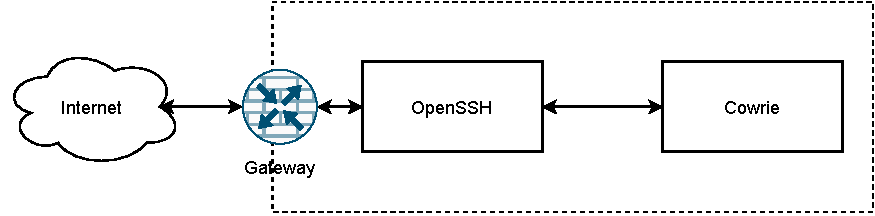
\includegraphics{figures/sshd-honeypot.pdf}
    \caption[Architecture of OpenSSH and Cowrie]{
        Architecture of OpenSSH and Cowrie (derived from \cite{vetterl2020}).
        A NAT rule forwards the communication from port 22.
        Only the sshd daemon is accessible from extern.
    }
    \label{fig:cowrie-fix}
\end{figure}

For instance, the latest OpenSSH version $8.8P1$\footnote{\href{https://github.com/openssh/openssh-portable/commit/bf944e3794eff5413f2df1ef37cddf96918c6bde}{OpenSSH 8.8P1} on GitHub} is used.
The implementation is based on \citet{vetterl2020} version $6.3P1$\footnote{\href{https://github.com/amv42/sshd-honeypot/commit/f58830161002baec9d3ed218e78ddb06b0d40a23}{sshd-honeypot} on GitHub}.
As mentioned beforehand, due to major differences between both versions, a smooth transition is unattainable without modifications.
Fortunately, the basic idea to morph OpenSSH into an intermediary instance stays the same.

In total, the connection and user authentication layer has been modified.
These are the following steps required to change the sshd daemon:

\begin{itemize}
    \item User authentication layer: permit any connection to communicate to Cowrie without an authentication running in front of it.
    \item Connection layer: create a separate channel to communicate with the attacker that forwards the packets to Cowrie.
    \item Connection layer: handle the communication with Cowrie in a new channel separated from others.
\end{itemize}

The first step is to tweak the authentication to permit any session to forward an incoming connection to Cowrie (\autoref{lst:openssh-auth}).
Initially, it checks each session to see if the chosen authentication method returns true.
In order to skip the authentication process, the server must return true for any client that tries to connect to the honeypot.
Therefore, the authentication method has to be overridden in the main method and the allowed user method that checks if the user is permitted to log in.
The authentication process validates if a connection to Cowrie is successful and returns true.
In case of failure, the authentication would fail, resulting in a loss of connection for the client.
Next, the libssh library expects a different integer for a successful authentication; therefore, the result is converted to the expected format.
The allowed user method is changed to return true for any user trying to connect to the honeypot.
Cowrie continues the authentication process and communicates with the attacker.

\begin{figure}
    \lstinputlisting[language=c, caption={[Tweaked OpenSSH authentication]Tweaked OpenSSH authentication to connect to Cowrie. Only the essential code parts to change the authentication method have been added.}, label={lst:openssh-auth}]{listings/auth-passwd.c}
\end{figure}

Second, the communication has to be forwarded to the honeypot (\autoref{lst:openssh-channel}).
In OpenSSH, communications are handled in channels as seen beforehand in \autoref{sec:openssh}.
Technically, the sshd daemon opens a SOCKS connection for each session to communicate with the client.
SOCKS is a network protocol to exchange packets between servers and clients.
The sshd daemon needs a separate channel to store the attacker's session and forward packets to communicate with Cowrie.
The channel is implemented in version $6.3P1$ and can be used in $8.8P1$ with minor adaptions.
The method validates if the Cowrie channel is open and writes the new packets into the buffer.
In the main method, when sshd is started, the channel is created, and a connection to the running Cowrie instance is opened to forward a new session.
If Cowrie is unavailable, the startup will fail; thus, it has to run prior to the sshd daemon.

\begin{figure}
    \lstinputlisting[language=c, caption={[Tweaked OpenSSH channel]Tweaked OpenSSH channel to connect to Cowrie. Only the essential code parts to change the authentication method have been added.}, label={lst:openssh-channel}]{listings/channels.c}
\end{figure}

Lastly, the server loop responsible for connecting the client to the correct port must be modified.
It puts direct TCP/IP connections in the respective channel.
The connection layer handles multiple sessions simultaneously over a single user authentication layer.
Without this adaption, Cowrie would not receive any packet.
The function in \autoref{lst:openssh-serverloop} handles these connections.
For instance, it checks if TCP forwarding is allowed and if the port of Cowrie is defined.
Then, it connects the current session to the respective port.
The sshd daemon has to be adapted to start and set up the channel in the main method at startup.
In addition, the configuration has to be extended to configure the daemon to set the Cowrie IP address and the port.

After compiling the version, a brief test proved a valid connection to the sshd daemon.

\begin{figure}
    \lstinputlisting[language=c, caption={[Tweaked OpenSSH server loop]Tweaked OpenSSH server loop to connect to Cowrie. Only the essential code parts to change the authentication method have been added.}, label={lst:openssh-serverloop}]{listings/serverloop.c}
\end{figure}

\section{Experiment 2: Avoid fingerprinting of Cowrie}

The last experiment to conclude this chapter is to test if the concept helps to disguise Cowrie and avoid fingerprint activities based on a custom local string version and key exchange initialization message.

For instance, \citet{vetterl2020} original $6.3P1$ sshd-honeypot and the newly implemented version $8.8P1$ will be used for this experiment.
The forwarding communications are handled by an unmodified Cowrie version $2.3.0$ running in a Docker environment.
The version $6.3P1$ has been tested in heiCLOUD on a Debian 9 Jessie distribution, whereas the version $8.8P1$ with our latest adaption has been tested on a Debian 10 Buster.
In addition, both versions are validated locally in an encapsulated environment.
The clients to test the two concepts are a standard OpenSSH $8.8.P1$ and the modified version with custom local version string and key exchange initialization message to fingerprint honeypots.

The standard client's requests do not result in a bad packet length exception for both servers.
This behavior reflects an original sshd communication and represents a successful test.
The requests from the modified client are successful on the latest version, whereas the older server $6.3P1$ had problems with new encryption and host key algorithms.
A successful connection to the original server from \citet*{vetterl2020} could be recreated by using the $7.3P1$ version.
This version has been used to verify Cowrie beforehand.
The concept can forward any related packet to Cowrie and hide the generic weakness of TwistedConch.
Therefore, whether Cowrie can be disguised to prevent any fingerprint activities with the help of OpenSSH has been answered successfully.
This section can confirm this assumption based on the reproduction and implementation of the concept.
On the other side, Cowrie receives the connection and log information (\autoref{lst:log-cowrie}).
However, one downside is the connection loss due to timeout restrictions.
This issue is a minor bug and could be fixed in the future.

In conclusion, this experiment has shown that the initial idea of hiding Cowrie in the background and directing the communication through OpenSSH prevents fingerprint activities of an adversary.
In addition, it has shown that protocol implementations change rapidly to adapt to new security standards, leading to outdated honeypots.

\begin{figure}
    \lstinputlisting[language={}, caption={[Cowrie log information]Cowrie log information. The new connection from this experiment has been acquired. Cowrie fetched information about the local string version and kex message.}, label={lst:log-cowrie}]{listings/cowrie.log}
\end{figure}

\section{Discussion}

Depending on the interaction level, honeypots will always deviate from production instances.
As seen in the two experiments beforehand, detecting a generic weakness is doable in a respective time, as well as mitigating it.
Thus, finding and fixing the weaknesses of honeypots becomes a continuous cycle.
However, this chapter also outlined the importance of the libraries that are used.
TwistedConch is the bottleneck of Cowrie, and it is updated\footnote{Based on the lastest GitHub commit of the Python library} frequently.
Libraries that reimplement protocols have to be always up-to-date.
In conclusion, such libraries should be chosen carefully to avoid bugs that leave harmful information to attackers.

\begin{figure}
    \centering
    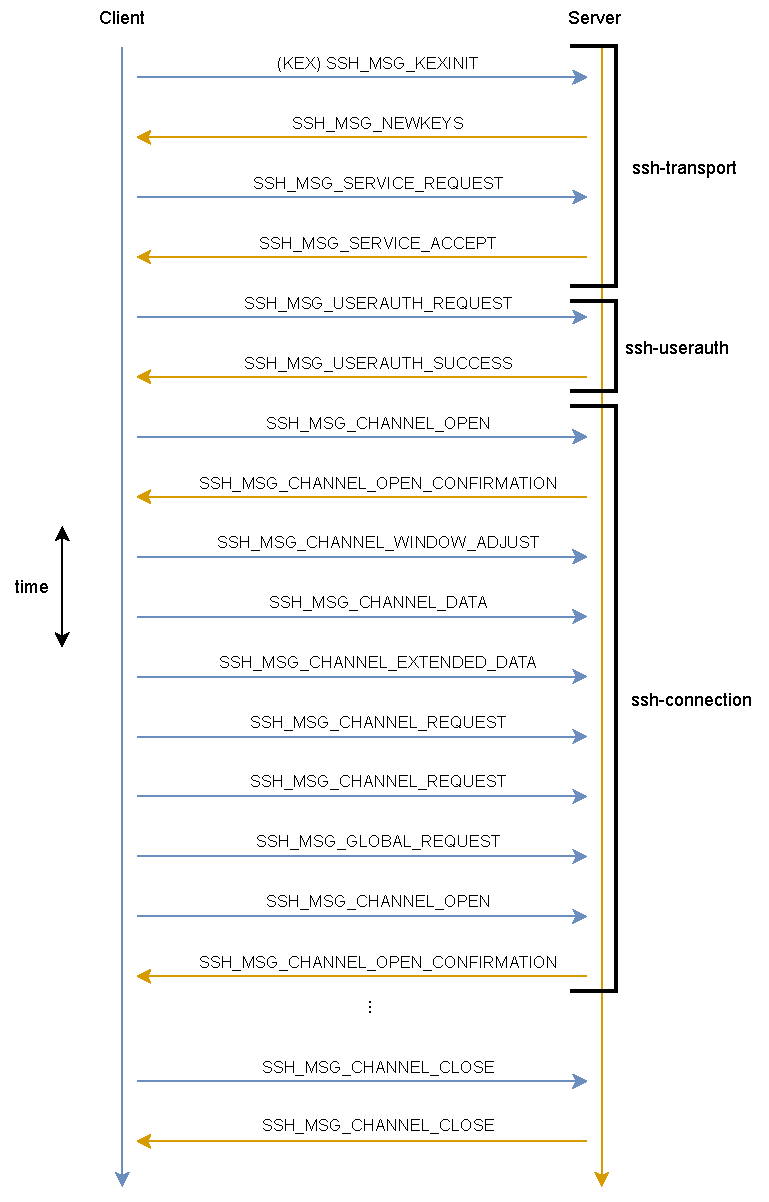
\includegraphics{figures/ssh-flow-diagram.pdf}
    \caption[OpenSSH sample session flow diagram]{
        OpenSSH sample session flow diagram (derived from \cite{openssh2007}).
        In addition, the right side indicates the layers that are responsible for handling the messages.
    }
    \label{fig:openssh-flow-diagram}
\end{figure}